\documentclass[13pt]{report}
\usepackage[a4paper, total={6in, 10in}]{geometry}

\usepackage[utf8]{inputenc}
\usepackage{enumerate}
\usepackage{tikz}
\usepackage{pgfplots}
\usetikzlibrary{plotmarks}
\usepackage{amssymb}
\usepackage{xcolor}
%\usepackage{enumitem}
\usepackage{listings}
\usepackage{polynom}
\usepackage{amsmath}
\usepackage{bm}
\renewcommand{\thesection}{\arabic{section}}
\renewcommand\theparagraph{\thesubsubsubsection.\arabic{paragraph}} % optional; useful if paragraphs are to be numbered

\usepackage{graphicx}
\usepackage{physics}
\graphicspath{ {images/} }

\addcontentsline{toc}{chapter}{Bibliography}
\renewcommand\bibname{References}

\renewcommand{\thesection}{\arabic{section}}
\renewcommand\theparagraph{\thesubsubsubsection.\arabic{paragraph}} % optional; useful if paragraphs are to be numbered

\setlength{\parindent}{10pt}
\newcommand{\forceindent}{\leavevmode{\parindent=1em\indent}}
%\linespread{1.5}
\usepackage{setspace}
\doublespacing
\setcounter{secnumdepth}{5}


\begin{document}
	
\begin{titlepage}
\centering
	\vspace{2cm}
	{\huge\bfseries Report of Project of Semester S1: Nonparametric method for image analysis \par}
	\vspace{2cm}
	{\Large\itshape Students:\\
		Loc Thi Thuy Linh\\
		Nguyen Duc Tho\par}
	\vfill
	supervised by\par
	\large Nghiem Thi Phuong \& Tran Giang Son\\
	ICT Department, USTH\par
	\vfill
% Bottom of the page
	{\large \today\par}
\end{titlepage}	
\tableofcontents{}
\newpage
\section{Introduction}
\subsection{Introduce to clustering}

\forceindent Cluster analysis or clustering is a very important technology in Data Mining. It divides the datasets into clusters which are collections of data objects with common characteristics based on the computation of data information.

Clustering problems come up in many different applications consisting data mining and knowledge discovery, data compression and vector quantization, and pattern recognition and pattern classification. There are several commonly used clustering algorithms, such as K-means, CLARANS, STING, CLIQUE, and CURE.  %Them trich dan cac ung dung


\subsection{Why does clustering be used?}

\subsection{How does clustering work?}

\subsection{Clustering categories}
Clustering algorithms may be classified as listed below:\\
Exclusive Clustering \\
Data are grouped in an exclusive way, so that if a certain datum belongs to a definite cluster then it could not be included in another cluster\\
Overlapping Clustering \\
On the contrary the second type, the overlapping clustering, uses fuzzy sets to cluster data, so that each point may belong to two or more clusters with different degrees of membership.In this case, data will be associated to an appropriate membership value.\\
Hierarchical Clustering \\
a hierarchical clustering algorithm is based on the union between the two nearest clusters. The beginning condition is realized by setting every datum as a cluster. After a few iterations it reaches the final clusters wanted\\\
Probabilistic Clustering\\
This one use a completely probabilistic approach


\section{K-means}

\subsection{What?}

\subsection{Why?}

\subsection{How?}

\subsection{Advantages and disadvantages}
%lead to the next part


\section{Non-parametric: Meanshift}

\subsection{What?}
\subsubsection{Clustering and Modes of Probability Density Function}
Mean shift  is a popular non-parametric clustering algorithm based on the
idea of associating each data point to a mode of the underlying probability density
function\textsuperscript{2.1}.Meanshift is a powerful tool for us in this case although the idea behind it is very simple. {\linebreak}

Assuming that we have a dataset of students and corresponding mark for each of them 
in final exam as the table below. How do we categorize these students into groups (clustering) base on their marks?
\begin{center}
 \begin{tabular}{||c c c||} 
 \hline
 No & Student & Mark \\ [0.5ex] 
 \hline\hline
 1 & S1 & 5.0 \\ 
 \hline
 2 & S2 & 4.0 \\
 \hline
 3 & S3 & 4.5 \\
 \hline
 4 & S4 & 5.7 \\
 \hline
 5 & S5 & 6.0 \\ 
  \hline
 6 & S6 & 9.0 \\ 
  \hline
 7 & S7 & 8.7 \\ 
  \hline
 8 & S8 & 9.5 \\ 
 [1ex] 
 \hline
\end{tabular}
\end{center}

Imagine that the set of marks was sampled from a probability distribution. We seek for the modes of  the underlying distribution for this set of marks. Number of modes corresponds to the number of groups of students.
\pgfplotsset{grid style={dashed,gray}}
\pgfplotsset{minor grid style={dashed,red}}
\pgfplotsset{major grid style={dotted,green!50!black}}

%Probability plot
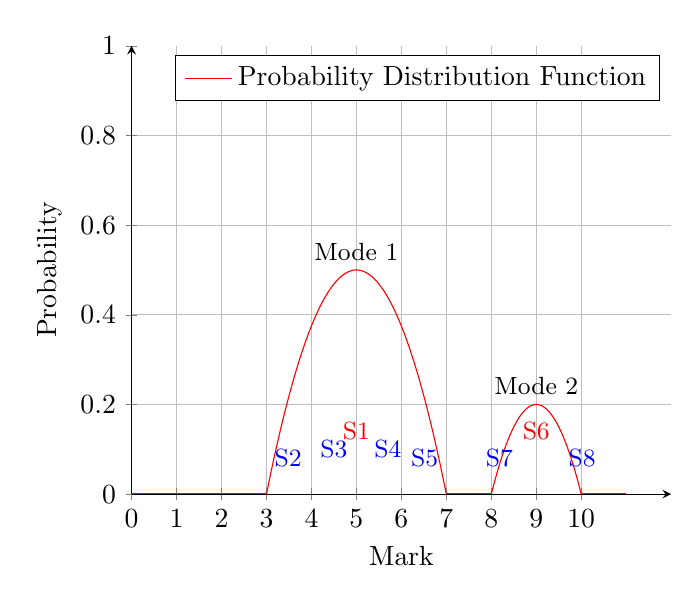
\begin{tikzpicture}
	\begin{axis}[
	axis lines=left,
	xtick={0,1,...,10},ytick = {0,0.2,...,1},
	grid=both,
	xlabel = {Mark},
	ylabel = {Probability}
	]
		%First Mode
		\addplot [
		domain=3:7,
		samples=100,
		color=red,
		]
		{-0.125*x^2 + 1.25*x - 2.625};
		
		\addplot [
		 domain=0:3,
		 samples=10, 
		 color=red,
		 ]
		 {0.002};
		 \addplot [
		 domain=7:8,
		 samples=10, 
		 color=red,
		 ]
		 {0.002};
		 \addplot [
		 domain=10:11,
		 samples=10, 
		 color=red,
		 ]
		 {0.002};
		 \addplot [
		domain=0:12, 
		samples=2,
		color = white
		]
		{1};
		%Second mode
		\addplot [
		domain=8:10, 
		samples=100, 
		color=red,
		]
		{-0.2*x^2 + 3.6*x - 16};
		 
		 %First Mode
		
		\draw[red,fill,thick] (50,50) circle (0.05cm);
		\node[black,above] at (axis cs:5,0.5){\small{Mode 1}};
		 %S1
		\draw[red,thick] (50,4) circle (0.2cm);
		\node[red,above] at (axis cs:5,0.1){\small{S1}};
		 %S2
		\draw[blue,thick] (40,4) circle (0.2cm);
		\node[blue,left] at (axis cs:4,0.08){\small{S2}};
		 %S3
		\draw[blue,thick] (45,4) circle (0.2cm);
		\node[blue,above] at (axis cs:4.5,0.06){\small{S3}};
		 %S4
		\draw[blue,thick] (57,4) circle (0.2cm);
		\node[blue,above] at (axis cs:5.7,0.06){\small{S4}};
		 %S5
		\draw[blue,thick] (60,4) circle (0.2cm);
		\node[blue,right] at (axis cs:6,0.08){\small{S5}};
		
		 %Second Mode
		 
		 \draw[red,fill,thick] (90,20) circle (0.05cm);
		 \node[black,above] at (axis cs:9,0.2){\small{Mode 2}};
		 %S6
		\draw[red,thick] (90,4) circle (0.2cm);
		\node[red,above] at (axis cs:9,0.1){\small{S6}};
		 %S7
		\draw[blue,thick] (87,4) circle (0.2cm);
		\node[blue,left] at (axis cs:8.7,0.08){\small{S7}};
		 %S8
		\draw[blue,thick] (95,4) circle (0.2cm);
		\node[blue,right] at (axis cs:9.5,0.08){\small{S8}};
		
		%Legend
		\addlegendentry{Probability Distribution Function}
	\end{axis}
\end{tikzpicture}

As can be seen from the graph above, we have two groups of students correspond to two modes of probability density function. 
With Mode 1, we have first group which includes: S1, S2, S3, S4, S5.  Similarly, correspoding to Mode 2 is second group, which includes : S6, S7, S8. That's why we can use mode-seeking algorithms as a solution of Clustering problem.
\subsubsection{Gradient Ascent and Modes of Probability Density Function}
The Taylor series of a function f(x) is described by the equation \textsuperscript{[2.2]}:
\[
    f(x+a) = f(x) + \frac{f'(x)}{1!}a+\frac{f''(x)}{2!}a^2+\frac{f'''(x)}{3!}a^3+...+\frac{f^{(n)}(x)}{n!}a^n
\]
\[\Longrightarrow f(x+a) \approx f(x) + \frac{f'(x)}{1!}a =  f(x) + f'(x)a\]
with a: learning rate,  f'(x): derivative or gradient of f(x)\\
Back to previous example in 3.1.1, let's say f(x) is the probability density function. As the illustration of the below graph, from any point on the graph of f(x), we continously move a small step f'(x).a$>$0 (Gradient Ascent) until reaching a local mode of f(x).\\ 
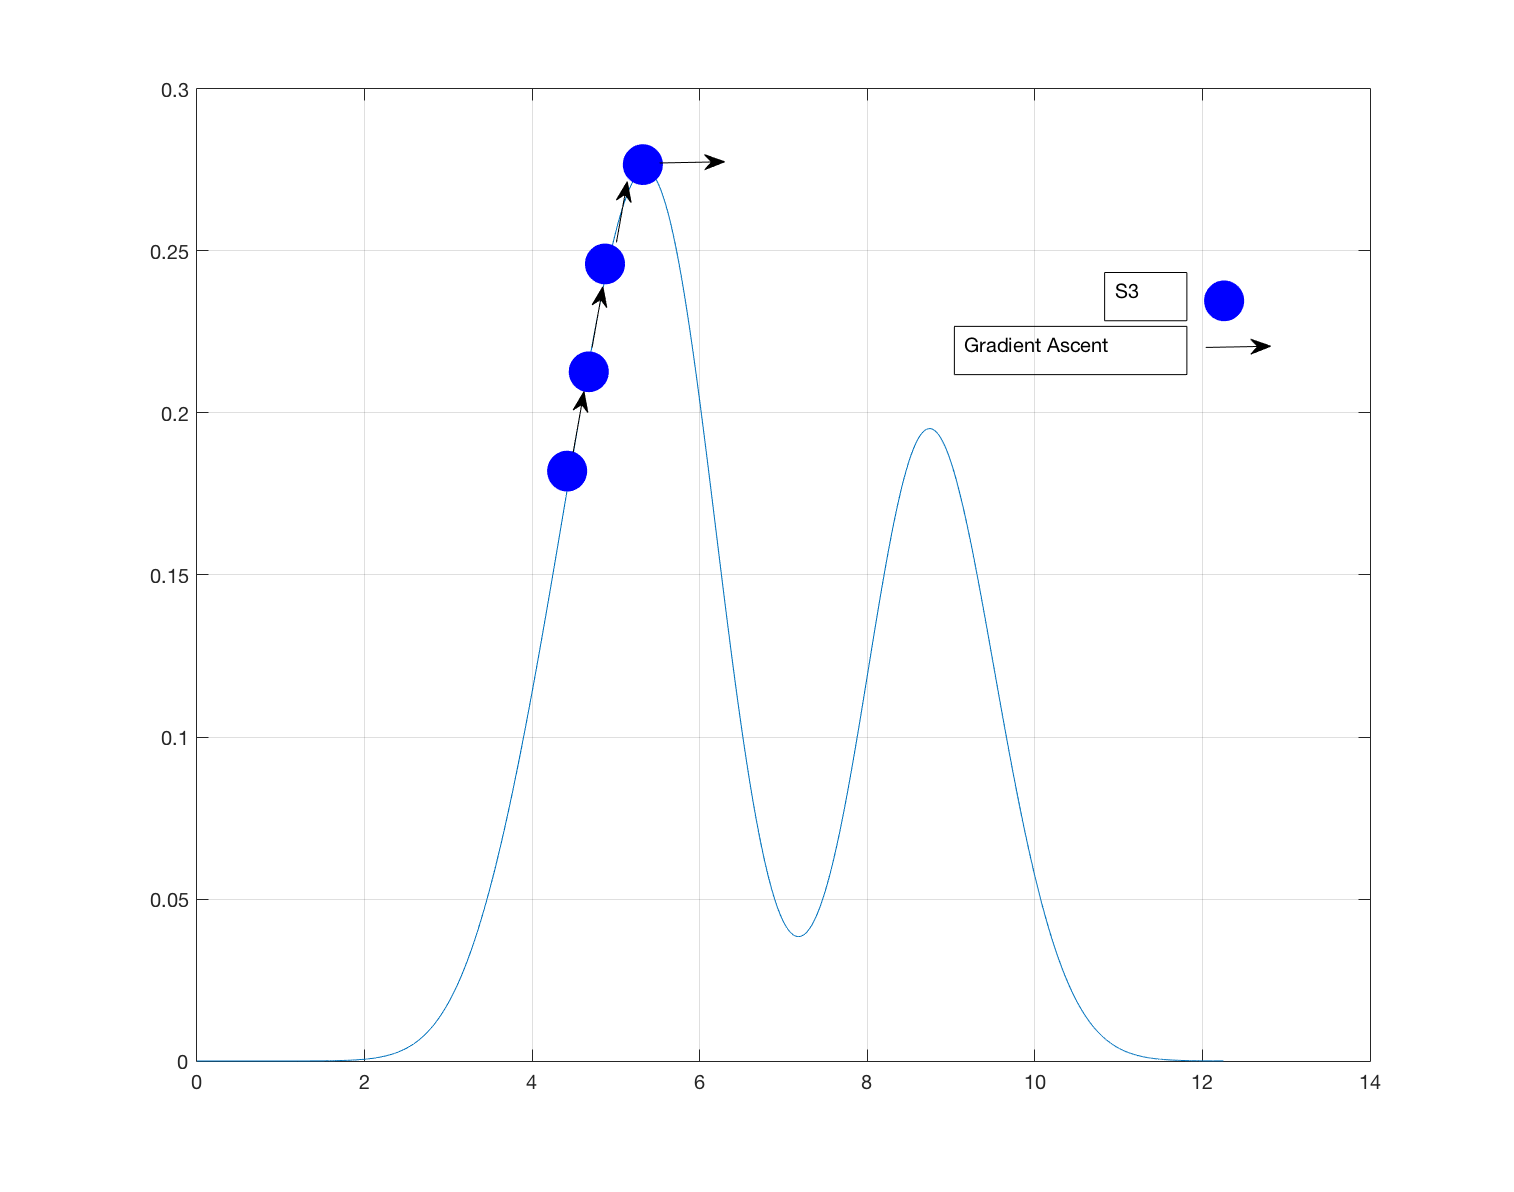
\includegraphics[width=\textwidth]{gradientAscent}
Important result: We can find modes of a probability density function by shifting a proper gradient ascent step from any point of that function. Generalization in n+1 dimensional space \[x=[x_0,x_1,...,x_n]\]
The pseudo code for Gradient Ascent algorithm of a dataset S of m points \[S = {x^0,x^1,...,x^m}\]
\fbox{\begin{minipage}{\textwidth}
\textit{
While(f'(x)a $>$ 0) \textbraceleft\\ 
For each x in S \textbraceleft
\[x := x + f'(x)a;\]\hspace{2.5cm}\textbraceright\\
\hspace{5cm}\textbraceright
}
\end{minipage}}

\subsubsection{Mean Shift Vector}

According to Domaniciu with given m data points x\textsuperscript{k} k = 1,...,m in the d-dimensional space R\textsuperscript{d}, the multivariate kernel density estimator (Probability Density Function) is f(x) and the mean shift vector of f(x) is defined as:
	%\[f(x) = \frac{1}{n}\sum_{i=1}^{n}K_H(x-x_i)\]
	%(\norm{\vb{\frac{x-x^i}{h}}}^2})
	\[m(x) = \frac{\sum_{k=1}^{m}x^i{w(x^k) }}{\sum_{k=1}^{m}{w(x^k) }) }-x\]
with a bandwith constant h we have \[w(x^k) = exp(-\frac{\norm{\vb{{x-x^k}}}^2}{2{h}^2})\] is a Gaussian Kernel (For simplicity purpose, we only using Gaussian Kernel in this report)
\subsection{Why and How}
Domaniciu also shows that m(x) is propotional to the gradient of f(x): m(x) = f'(x).c with a constant c.\\ With the weighted mean \[\bar{m} = \frac{\sum_{k=1}^{m}x^i{w(x^k) }}{\sum_{k=1}^{m}{w(x^k) }) }\]The pseudo code of Gradient Ascent algorithm in 3.1.2 becomes:\\\\
\fbox{\begin{minipage}{\textwidth}
\textit{
While($\bar{m} > 0$) \textbraceleft\\ 
For each x in S \textbraceleft
\[x := x + m(x)\]\hspace{5cm}or\[x:= \bar{m}\]\hspace{2.5cm}\textbraceright\\
\hspace{5cm}\textbraceright
}
\end{minipage}}
\\\\Instead of computing the gradient of f(x), which is sometimes impossible, now we can compute the weighted mean $\bar{m}$, that is defenitely doable. 

\subsection{Advantages and disadvantages}

2.2 https://web.stanford.edu/class/cs168/l/l5.pdf
\section{Evaluation}

\begin{enumerate}[(a) ]
\item What is evaluation? Convergence(performance) | accuracy | Complexity
\item Dataset (name, source, type, image size ....)
\item Computer test configuration
\item Program language
\item Results (time | number of cluster | accuracy) ~~~> describe detail.
\item Comparison of the two methods
\end{enumerate}
\section{Conclusion}
\begin{thebibliography}{1}
	\bibitem{notes} John W. Dower {\em Readings compiled for History
		21.479.}  1991.
	\bibitem{impj}  The Japan Reader {\em Imperial Japan 1800-1945} 1973:
	Random House, N.Y.
	\bibitem{norman} E. H. Norman {\em Japan's emergence as a modern
		state} 1940: International Secretariat, Institute of Pacific
	Relations.
	\bibitem{fo} Bob Tadashi Wakabayashi {\em Anti-Foreignism and Western
		Learning in Early-Modern Japan} 1986: Harvard University Press.
\end{thebibliography} 

\end{document}